%%%%%%%%%%%%%%%%%%%%%%%%%%%%%%%%%%%%%%%%%%%%%%%%%%%%%%%%%%%%%%%%%
% !TEX root = interimreport.tex
\clearpage
\chapter{TESTING}\label{Ch10}
%%%%%%%%%%%%%%%%%%%%%%%%%%%%%%%%%%%%%%%%%%%%%%%%%%%%%%%%%%%%%%%%%
LLVM-lit coordinates the testing procedure. The comment lines that start with “RUN” call other programs via LLVM-lit. LLVM-lit also gives the output of a program to another program as an input.

FileCheck, as the name implies, controls the checking process. It basically compares the file and the corresponding lines of the output. It is used with CHECK-* command.

Regression testing is a core part of LLVM because of its size and active development. To make sure newly added features don’t break the already present functionality it is a must to both build functionality and its corresponding tests.

\section{MC Test}
LLVM-MC is an abstracted assembler integrated with the Compiler. \cite{Lattner2010Apr}

Before adding a new instruction, check its byte sequence. LLVM-MC is going to be used to get the output. 

Here is a working test file:

\begin{lstlisting}
\# RUN: llvm-mc %s -triple=riscv32 -riscv-no-aliases -show-encoding \ 
\# RUN: 	| FileCheck -check-prefixes=CHECK-ASM,CHECK-ASM-AND-OBJ %s 
\# RUN: llvm-mc -filetype=obj -triple=riscv32 < %s \ 
\# RUN: 	| llvm-objdump -M no-aliases -d -r - \ 
\# RUN: 	| FileCheck -check-prefixes=CHECK-ASM-AND-OBJ %s 

\# CHECK-ASM-AND-OBJ: shlxor s2, s2, s8 
\# CHECK-ASM: encoding: [0x33,0x59,0x89,0x81] 
shlxor s2, s2, s8
\end{lstlisting}


The first RUN command sequence results in the output given in figure \ref{fig:result_of_first_run_command}.
\begin{figure}
    \centering
    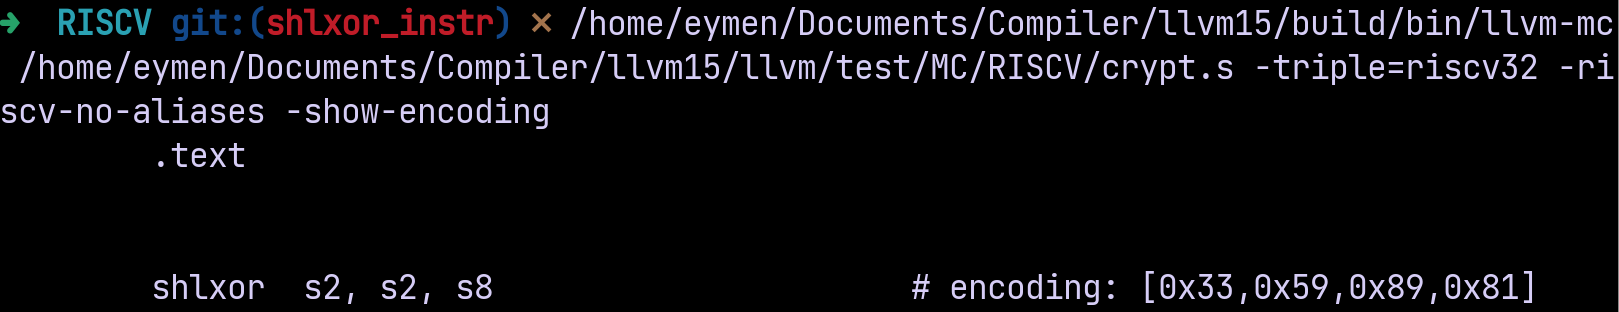
\includegraphics{testing/result_of_first_run_command.png}
    \caption{Result of first "RUN" command}
    \label{fig:result_of_first_run_command}
\end{figure}

Here, FileCheck is checking both the Assembly encoding and the string as it was provided with the prefixes: CHECK-ASM, CHECK-ASM-AND-OBJ.


The second RUN sequence with only the llvm-mc part spits out an ELF object which itself isn’t useful. The console output can be seen in figure \ref{fig:result_of_second_run_command}.
\begin{figure}
    \centering
    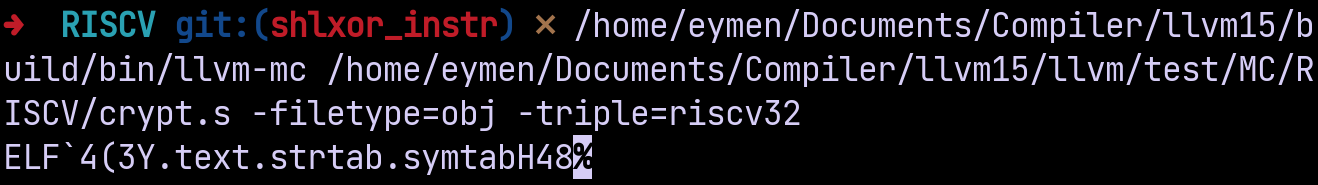
\includegraphics{testing/result_of_second_run_command.png}
    \caption{Result of second "RUN" command}
    \label{fig:result_of_second_run_command}
\end{figure}

By using the pipe ‘|’ operator like in Shell, we can tell LLVM-lit to feed another program with the output of a program. An example is given in figure \ref{fig:use_of_pipe_operator}.
\begin{figure}
    \centering
    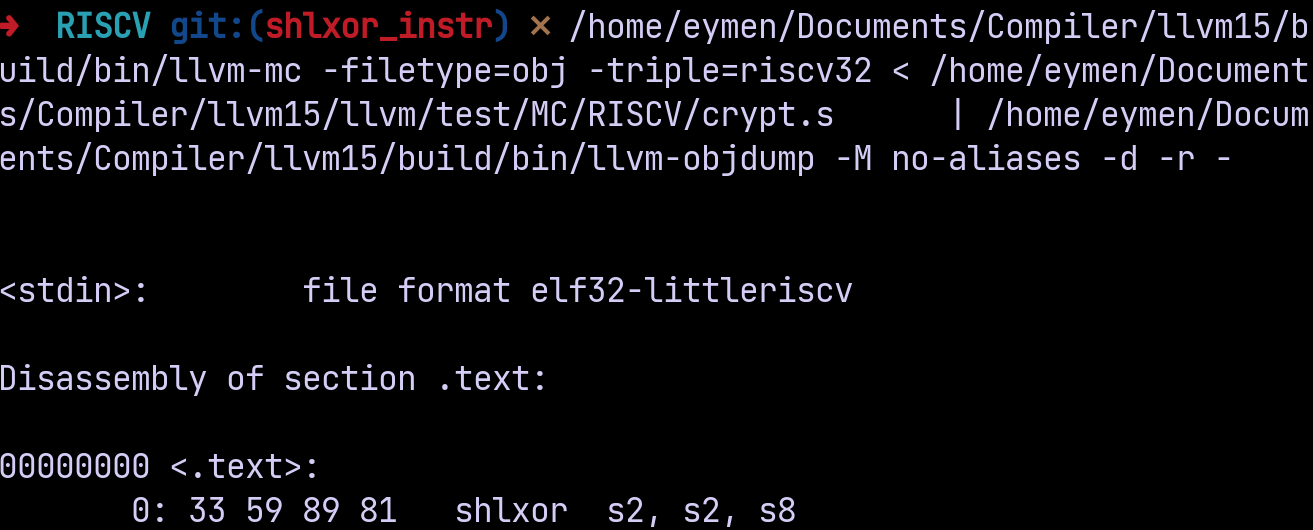
\includegraphics{testing/use_of_pipe_operator.png}
    \caption{Use of pipe operator}
    \label{fig:use_of_pipe_operator}
\end{figure}

Since we observed the outputs of the commands, we can make sense of what FileCheck is checking. Here in the second RUN sequence, FileCheck is provided only with CHECK-ASM-AND-OBJ and therefore it does not check the CHECK-ASM line. It seems that the object dump resulted the correct string.

In figure \ref{fig:output_for_successfully_passed_test} we can observe that the test is passed:

\begin{figure}
    \centering
    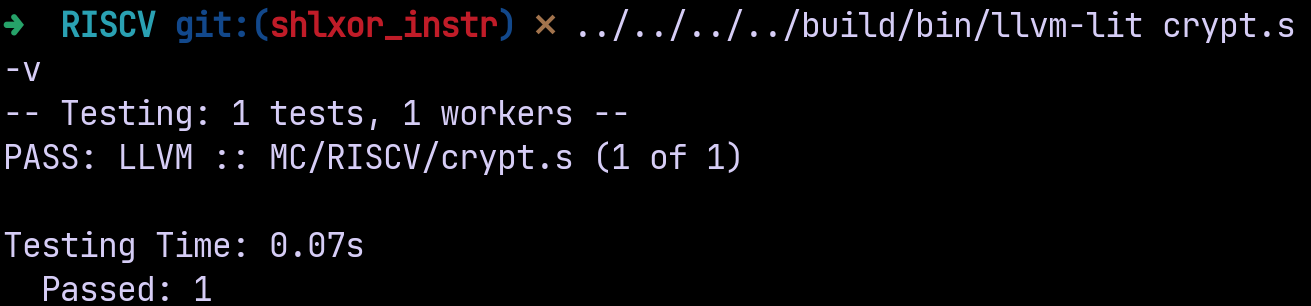
\includegraphics{testing/output_for_successfully_passed_test.png}
    \caption{Output for successfully passed test}
    \label{fig:output_for_successfully_passed_test}
\end{figure}

Another complexity LLVM-lit handles is the path of our compiled binaries. The test case is free of the paths and \%s placeholders are populated by LLVM-lit.

\section{Writing the MC Test}
LLVM-MC can be run before writing the test to see the encoding or hand-coding is also possible. It would be great if it was automatic like the llc test cases.

The header of the MC test can be used, if prefixes other than the present one are needed, add them to the –check-prefixes= side and make sure to use them in the file.

\section{LLC/CodeGen Test}
llc tests are more familiar since they check how an .ll produces Assembly-like (MCInst) strings. Instead of the manual checking, this tool can be used and batch-testing can be done.

Here is an example of the LLVM-IR code implemented for the SHLXOR instruction that we want. As it can be seen from its signature, it is a function taking two 32 bit integers and returning one. It takes one input, shifts it left by one and assigns it to a variable \%1. \%1 is then XOR’ed with the second input and the result is returned.

\begin{lstlisting}
; RUN: llc -mtriple=riscv32 -verify-machineinstrs < %s \ 
; RUN: | FileCheck %s -check-prefix=RV32R 


define i32 @shlxor(i32 %a, i32 %b) nounwind { 
%1 = shl i32 %a, 1 
%2 = xor i32 %1, %b 
ret i32 %2 
} 
\end{lstlisting}

In contrast to MC tests, we can use a utility script as shown in figure \ref{fig:command_for_using_utility_script} to generate the expected result for us.

\begin{figure}
    \centering
    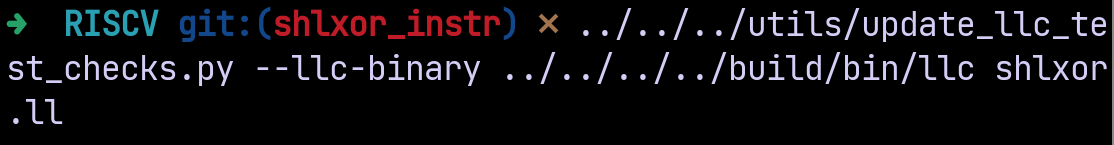
\includegraphics{testing/command_for_using_utility_script.png}
    \caption{Command for using utility script}
    \label{fig:command_for_using_utility_script}
\end{figure}

The script is located at llvm/utils/

The llc test file is populated with FileCheck lines as seen in figure \ref{fig:llc_test_file}.
\begin{figure}
    \centering
    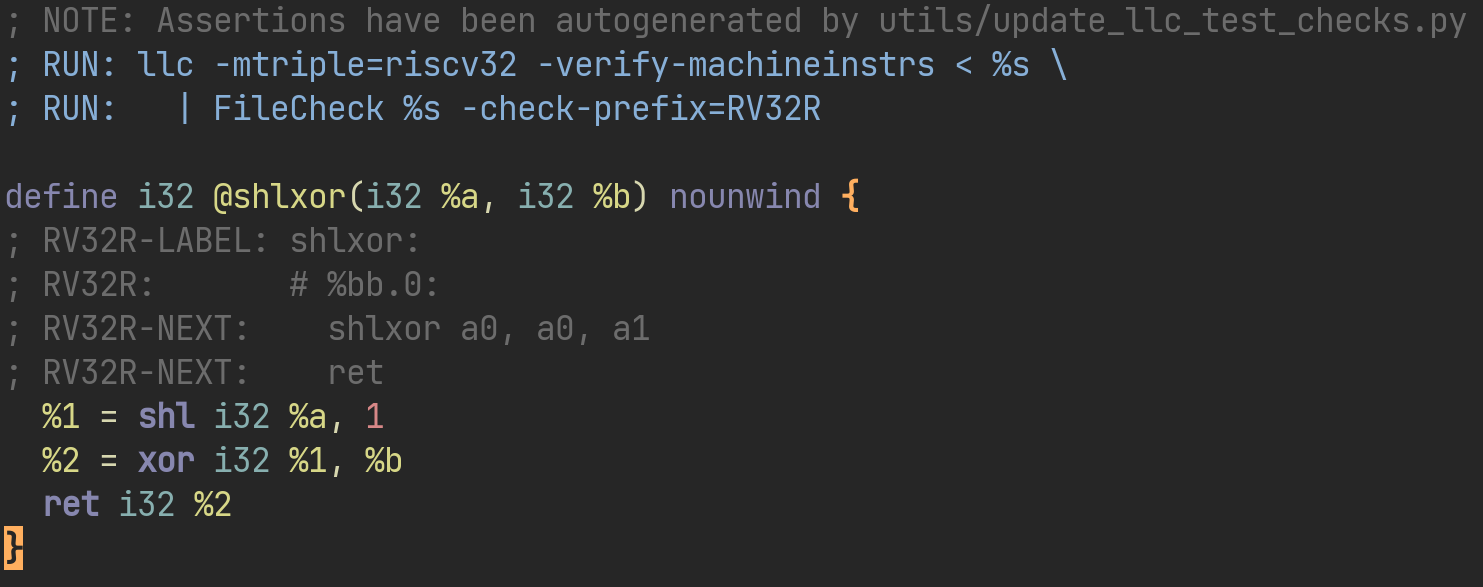
\includegraphics{testing/llc_test_file.png}
    \caption{LLC test file}
    \label{fig:llc_test_file}
\end{figure}

We can observe that our newly added SHLXOR instruction is recognized and placed in the check lines. When LLVM-lit is run with the test file, the test is passed as the new instruction is implemented. Output for a successful test is given in figure \ref{fig:output_for_passed_ll_test}.
\begin{figure}
    \centering
    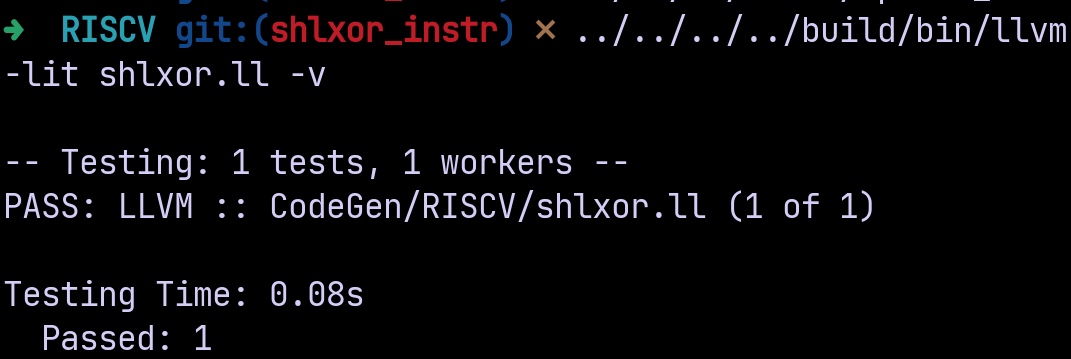
\includegraphics{testing/output_for_passed_ll_test.png}
    \caption{Output for passed .ll test}
    \label{fig:output_for_passed_ll_test}
\end{figure}

\section{Running Tests}
For running the tests, we should run the following command.

\begin{lstlisting}
build/bin/llvm-lit llvm/test/PATH-OF-FILE -v
\end{lstlisting}
